\begin{figure}[ht]
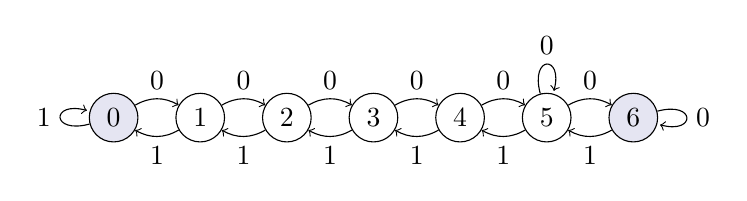
\begin{tikzpicture}
	\definecolor{light-gray}{rgb}{0.9,0.9,0.95}
   
	\node[shape=circle,draw=black, fill=light-gray] (0) at (0, 0) {0};
   	\node[shape=circle,draw=black] (1) at (1.1, 0) {1};
   	\node[shape=circle,draw=black] (2) at (2.2, 0) {2};
    \node[shape=circle,draw=black] (3) at (3.3, 0) {3};
    \node[shape=circle,draw=black] (4) at (4.4, 0) {4};
    \node[shape=circle,draw=black] (5) at (5.5, 0) {5};
    \node[shape=circle,draw=black, fill=light-gray] (6) at (6.6, 0) {6};
	
   	\draw[->, bend left=30] (0) edge node[above] {0} (1);
   	\draw[->, bend left=30] (1) edge node[above] {0} (2);
   	\draw[->, bend left=30] (2) edge node[above] {0} (3);
   	\draw[->, bend left=30] (3) edge node[above] {0} (4);
   	\draw[->, bend left=30] (4) edge node[above] {0} (5);
   	\draw[->, bend left=30] (5) edge node[above] {0} (6);

	\draw[->, loop above] (5) edge node[above] {0} (5);
	\draw[->, loop right] (6) edge node[right] {0} (6);

	\draw[->, bend left=30] (6) edge node[below] {1} (5);
    \draw[->, bend left=30] (5) edge node[below] {1} (4);
    \draw[->, bend left=30] (4) edge node[below] {1} (3);
    \draw[->, bend left=30] (3) edge node[below] {1} (2);
    \draw[->, bend left=30] (2) edge node[below] {1} (1);
    \draw[->, bend left=30] (1) edge node[below] {1} (0);
   
    \draw[->, loop left] (0) edge node[left] {1} (0);
\end{tikzpicture}
\caption{Grafo de transições do agente}
\end{figure}